% A chapter named 'Your first document' is created
\chapter{Componenten} \label{cha:componenten}


\section{Hoofdscherm} \label{sec:hoofdscherm}
\begin{figure}[h]
  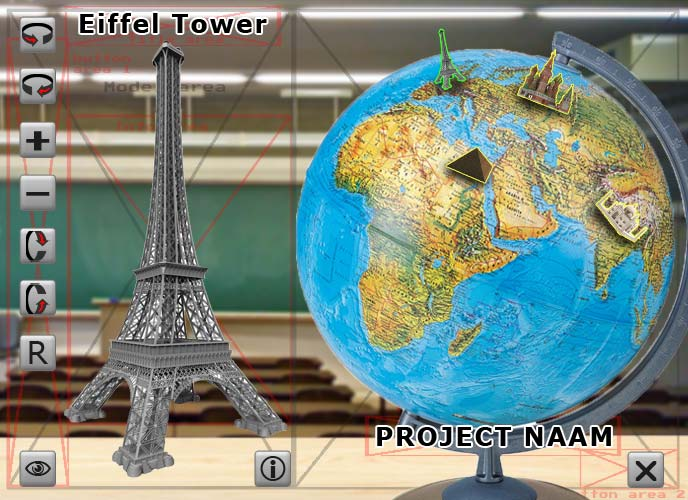
\includegraphics[width=130mm]{figs/components1.jpg}
  \caption{Componenten hoofdscherm \textit{(27-April-2014)}}
  \label{fig:components1}
\end{figure}

Het hoofdscherm is een reflectie van het camerabeeld dat wordt opgenomen. Dit scherm is wat de gebruiker hoofdzakelijk zal zien en bevat alle navigatie elementen. Het achterliggende transparante wireframe is hier slechts te zien ter verduidelijking, bij release van de applicatie zal deze niet  zichtbaar zijn. Een belangrijk aspect is dat de applicatie alleen bruikbaar is bij een specifieke wereldbol. De wereldbol is namelijk voorzien van speciale markering die dient om de positie van de 3D modellen op de bol aan te sturen.

\newpage
\section{Digitale componenten} \label{sec:digicomponents}
\begin{figure}[h]
  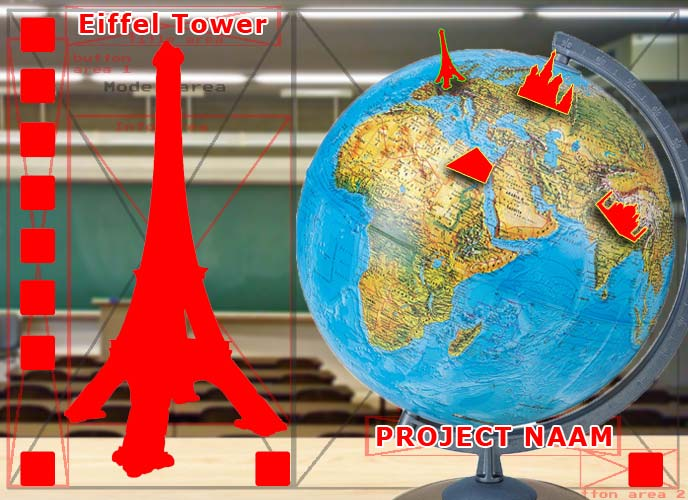
\includegraphics[width=130mm]{figs/components4.jpg}
  \caption{Digitale componenten (rood) \textit{(27-April-2014)}}
  \label{fig:digitals}
\end{figure}

In het \textbf{{\color{red}rood}} zijn alle elementen weergegeven die digitaal zullen worden weergegeven. Afhankelijk van de positie van de wereldbol zullen er 3D modellen worden weergegeven op de reflectie van de wereldbol op het scherm. Deze modellen draaien volledig mee met de assen van de wereldbol. Een geselecteerd model wordt gehighlight zodat het voor de gebruiker duidelijk is dat er iets is geselecteerd (In \cref{fig:digitals} heeft de Eiffel toren op de bol bijvoorbeeld een groene rand). 

\newpage
\section{Knoppen} \label{sec:buttons}
\begin{table}[h]
  \centering
  \caption{knoppen legenda}
  \label{tb:table}
  \begin{tabular}{crl}
    \toprule
    Button     & beschrijving   \\
    \midrule
    
\includegraphics[width=15px]{figs/button1.png}     & Pitch model rechtsom horizontaal   \\
    
\includegraphics[width=15px]{figs/button2.png}     & Pitch model linkssom horizontaal   \\
    
\includegraphics[width=15px]{figs/button3.png}     & Zoom in   \\
    
\includegraphics[width=15px]{figs/button4.png}     & Zoom uit   \\
    
\includegraphics[width=15px]{figs/button5.png}     & Yaw model naar onder   \\
    
\includegraphics[width=15px]{figs/button6.png}     & Yaw model naar boven   \\
    
\includegraphics[width=15px]{figs/button7.png}     & Reset model view   \\
    
\includegraphics[width=15px]{figs/button8.png}     & Toggle buttons aan/uit   \\
    
\includegraphics[width=15px]{figs/button9.png}     & Sluit applicatie   \\
    
\includegraphics[width=15px]{figs/button10.png}    & Toggle infoscherm aan   \\
    
\includegraphics[width=15px]{figs/button11.png}    & Toggle infoscherm uit   \\    
    \bottomrule
  \end{tabular}
\end{table}
\begin{figure}[h]
  \centering
  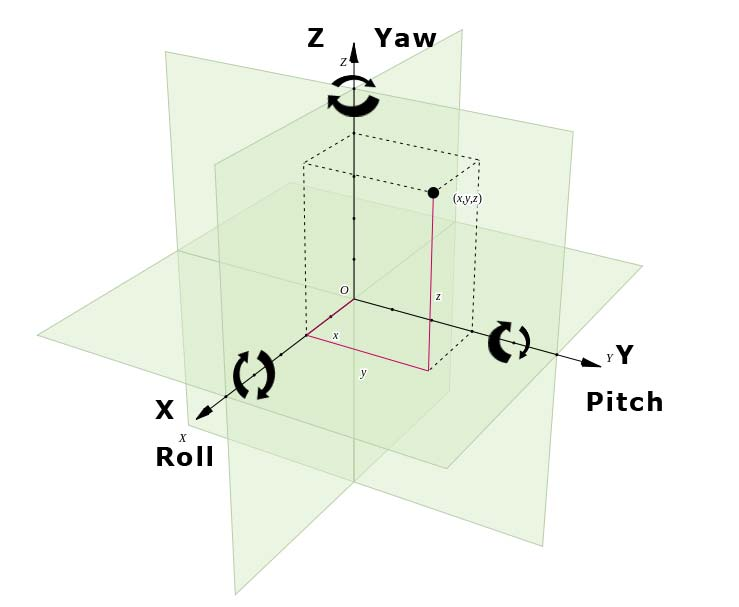
\includegraphics[width=70mm]{figs/terminology.jpg}
  \caption{XYZ axis beweging terminologie}
  \label{fig:termi}
\end{figure}

\newpage
\section{Infoscherm} \label{sec:infoscherm}
\begin{figure}[h]
  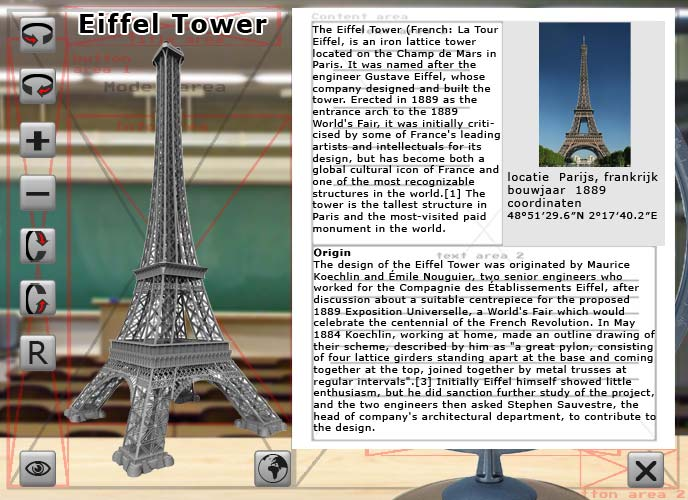
\includegraphics[width=130mm]{figs/components2.jpg}
  \caption{Componenten infoscherm \textit{(27-April-2014)}}
  \label{fig:components2}
\end{figure}
De 
\includegraphics[width=15px]{figs/button10.png} button laat een venster openen met informatie over het geselecteerde monument. Als dit scherm actief it, kan er geen monument worden geselecteerd van de wereldbol, het model links van het scherm kan nog wel worden gemanipuleerd. De gebruiker sluit het infoscherm door op de 
\includegraphics[width=15px]{figs/button11.png} button te drukken.

\newpage
\section{Afsluitscherm} \label{sec:exitscherm}
\begin{figure}[h]
  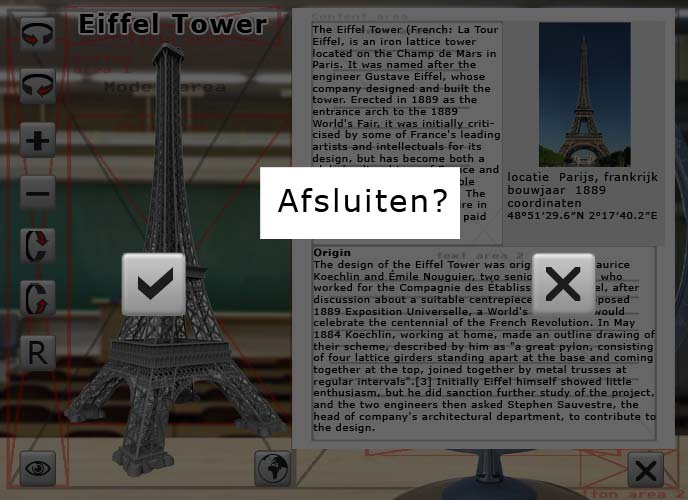
\includegraphics[width=130mm]{figs/components3.jpg}
  \caption{Componenten afsluitscherm \textit{(27-April-2014)}}
  \label{fig:components3}
\end{figure}
De gebruiker kan ten alle tijden de applicatie sluiten met de 
\includegraphics[width=15px]{figs/button9.png} button. Na het indrukken van de button verschijnt een prompt met de vraag om de applicatie te sluiten. De gehele navigatie wordt geblokkeerd zodat alleen antwoord op het prompt kan worden gegeven. De gebruiker kan kiezen om de applicatie te sluiten of terug te keren.